\chapter{Pruebas de multinormalidad}
Para rechazar la hipótesis de que el conjunto de datos provenia de una distribución normal multivariada se utilizaron gráficos de las distribuciones marginales, y se 
realizaron las pruebas de Maridas, y de Henze-Zirklers. Para todo el análisi se utilizó el paquete de $R$ MVN. Y también, al final se incluye el código implementado.

Primero analisando los gráficos QQ plot de la gráfica \ref{fig:qqplot} podemos ver que para las tres compañías difiere el valor teórico del cuantil de la distribución normal del valor del cuantil empírico de los datos tanto para las observaciones de las tres compañías. También nótese que para valores chicos, la distribución teórica sobrepasa a la distribución empírica, mientras que para valores grandes, la distribución empírica sobrepasa a la distribución teórica. Lo que nos da un indicio de que marginalmente las distribuciones podrían no distribuirse normalmente.

\begin{figure}[h]
	\centering
	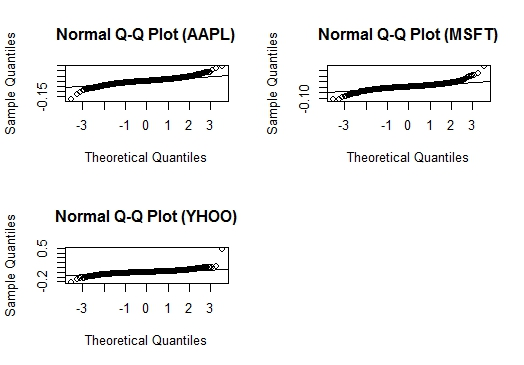
\includegraphics[width=1\linewidth]{Figuras/QQplot}
	\caption[Gráficos QQ]{Gráficos QQ plot.}
	\label{fig:qqplot}
\end{figure}
 
 Después, como se muestra en la gráfica \ref*{fig:histmarg}, si analizamos marginalmente el histograma empírico de los retornos de cada compañía podemos observar que la kurtosis parece ser mayor que el de una distribución normal, lo cual se puede verificar al calcular los momentos muestrales, pues para la empresa apple se tiene un coeficiente de kurtosis de $5.986$, para Microsoft de $10.397$ y para yahoo de $56.217$. También el sesgo muestral de cada compañía es de $-0.178$, $0.497$ y de $2.482$ respectivamente.  
 
 \begin{figure}[h]
 	\centering
 	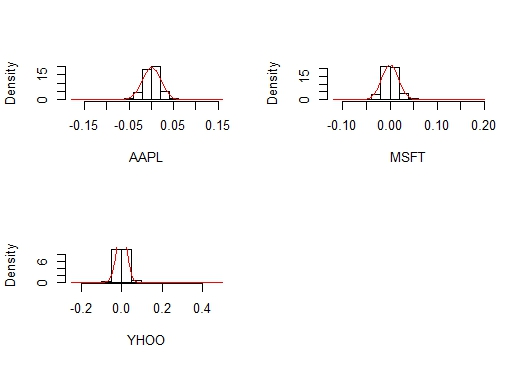
\includegraphics[width=1\linewidth]{Figuras/histmarg}
 	\caption{Histogramas}
 	\label{fig:histmarg}
 \end{figure}

Dicho lo anterior, tenemos evidencia para creer que marginalmente las distribuciones de los retornos de cada compañía no provienen de una distribución normal, lo cual podemos probar mediante la prueba Shapiro-Wilk del paquete $stats$ de $R$.

Implementando la prueba Shapiro-Wilk para cada conjunto de datos obtenemos que la estadística de prueba $w$ para Apple es de $0.94$, de $0.9065$ para Microsoft, y de $.8427$ para Yahoo; todas las pruebas tienen un valor $p$ de prácticamente cero, lo que rechaza la hipótesis de normalidad para los tres casos.

Una vez teniendo que las distribuciones marginales no provienen de una distribución normal, tenemos motivos para creer que la distribución conjunta de las tres compañías no es normal multivariada, pues de serlo sus distribuciones marginales debieran ser normales, lo cual se prueba a continuación.


Como se mencionó anteriormente, después de aplicarse la prueba de Marida, se obtuvo que el estadístico de prueba para el sesgo tiene un valor de $18.1$ , mientras que el de Kurtosis de $141.41$, ambos estadísticos mostraron un valor $p$ de cero, con lo cual se rechaza la hipótesis de que los datos provienen de una distribución normal multivarada.

Para la prueba Henz-Zirklers se obtuvo un estadística de prueba de 40.83, e igualmente un valor $p$ de cero con lo que igualmente se rechaza la hipótesis de que los datos fueron generados por una distribución normal multivariada. 

Por lo tanto, si juntamos los gráficos marginales y las pruebas realizadas, concluimos que el conjunto de datos no fue generado por una distribución normal multivariada.


\subsection{Código en R para la prueba de multinormalidad}

\lstinputlisting[language=R]{codigo/pruebas.r}

    